% Tipo de documento. En este caso es un art�culo, para folios A4, tama�o de la fuente 11pt y con p�gina separada para el t�tulo
\documentclass[a4paper,11pt,titlepage]{article}

% Carga de paquetes necesarios. OrdenesArticle es un paquete personalizado
\usepackage[spanish]{babel} 
\RequirePackage[T1]{fontenc}
\RequirePackage[ansinew]{inputenx} 
\usepackage[spanish,cap,cont,title,fancy]{OrdenesArticle}
\usepackage{array}
\usepackage{graphicx}
\usepackage{hyperref}
\usepackage{pifont}
\usepackage{listings}
\usepackage[usenames,dvipsnames]{color}
\usepackage{colortbl}
\usepackage{makeidx}
\hypersetup{bookmarksopen,bookmarksopenlevel=3,linktocpage,colorlinks,urlcolor=blue,citecolor=blue,
						linkcolor=blue,filecolor=blue,pdfnewwindow,
						pdftitle={Motor de indexaci�n}, 
						pdfsubject={Almacenamiento y Recuperaci�n de la Informaci�n}
						pdfauthor={Juan Andrada, Jose Domingo L�pez}}


% Macro para definir una lista personalizada 
\newenvironment{milista}%
{\begin{list}{\textbullet}%
{\settowidth{\labelwidth}{\textbullet} \setlength{\leftmargin}{\dimexpr\labelsep+\labelwidth+5pt}
\setlength{\itemsep}{\dimexpr 0.5ex plus 0.25ex minus 0.25ex}
\setlength{\parsep}{\itemsep}
\setlength{\partopsep}{\itemsep}
\addtolength{\topsep}{-7.5pt}
}}%
{\end{list}}


\begin{document}

% En las p�ginas de portada e �ndices, no hay encabezado ni pie de p�gina
\pagestyle{empty} 

% Se incluye la portada
\begin{titlepage}
	\begin{center}
  	{\LARGE UNIVERSIDAD DE CASTILLA-LA MANCHA} \\
  	\bigskip
  	{\Large ESCUELA SUPERIOR DE INFORM�TICA} \\
  	\vspace{20mm}
  	
\includegraphics[scale=0.45, keepaspectratio]{./images/esi_bw.png} \\
  	\vspace{20mm}
  	{\Huge \textbf{Almacenamiento y Recuperaci�n de la Informaci�n}}\\
  	\vspace{10mm}
  	{\LARGE \textsc{\textbf{M�dulo de importaci�n e indexaci�n de documentos}}}\\
  	\vspace{30mm}
  	\today
  	\vspace{40mm}
  	\begin{flushleft}
  		{\large Juan Andrada Romero}\\
  		\vspace{1mm}
  		{\large Jose Domingo L�pez L�pez}\\		
  	\end{flushleft}
	\end{center}
\end{titlepage}

% Se ajusta la separaci�n entre p�rrafos
\parskip=10pt
\pagestyle{fancy} 
% Aqui se incluyen los archivos .tex que forman el documento
\section{Introducci�n}
\subsection{Enunciado del problema}

\subsection{Dise�o elegido}
Para implementar la pr�ctica y, en concreto, este motor de indexaci�n, se utilizar� el lenguaje de programaci�n Python (\cite{Python}). 

Para implementar los elementos necesarios para la indexaci�n de documentos, como son el \textit{Posting$\_$File}, la tabla de documentos y el diccionario de t�rminos, se ha optado por utilizar una base de datos relacional, siguiendo el diagrama mostrado en la Figura \ref{BD}. Las tablas que se representan son:

\begin{milista}
	\item \textbf{dic}: implementa el diccionario de t�rminos. Tiene los campos \textit{term} y \textit{num$\_$docs}, que representan cada uno de los t�rminos encontrados, junto con el n�mero de documentos donde aparece cada t�rmino.
	\item \textbf{doc}: implementa la tabla de documentos. Tiene los campos \textit{id$\_$doc}, \textit{title} y \textit{path} para almacenar un identificador �nico de documento, el t�tulo del documento y la ruta del sistema donde se almacena una copia de dicho documento. 
	\item \textbf{posting$\_$file}: implementa el posting$\_$file. Contiene los campos \textit{term}, \textit{id$\_$doc} y \textit{frequency} para representar la frecuencia con la que aparece un t�rmino en un documento. Por tanto, el campo \textit{term} hace referencia a t�rminos del diccionario, y el campo \textit{id$\_$doc} hace referencia a los documentos de la tabla de documentos.
\end{milista}
\clearpage
\section{Decisiones de dise�o} \label{decisiones}

\subsection{Lenguaje de programaci�n y sistema operativo elegido}

Para implementar el sistema, se ha decidido utilizar el lenguaje de programaci�n Python (\cite{Python}). Se ha seleccionado este lenguaje de programaci�n ya que permite el uso de estructuras como diccionarios (tablas hash), listas, manejadores de archivos, llamadas al sistema, definici�n de patrones mediante expresiones regulares, etc. Dichos elementos han facilitado el desarrollo de este m�dulo del sistema, ya que Python los gestiona de una manera eficaz y permite su uso de uso de una manera sencilla.

Por otra parte, hemos elegido un sistema UNIX porque nos resulta m�s c�modo a la hora de implementar el sistema.

\subsection{Dise�o de la base de datos}

Para implementar los elementos necesarios para la indexaci�n de documentos, como son el \textit{Posting$\_$File}, la tabla de documentos y el diccionario de t�rminos, se ha optado por utilizar una base de datos relacional, siguiendo el diagrama mostrado en la Figura \ref{BD}. Las tablas que se representan son:

\begin{milista}
	\item \textbf{dic}: implementa el diccionario de t�rminos. Tiene los campos \textit{term} y \textit{num$\_$docs}, que representan cada uno de los t�rminos encontrados, junto con el n�mero de documentos donde aparece cada t�rmino.
	\item \textbf{doc}: implementa la tabla de documentos. Tiene los campos \textit{id$\_$doc}, \textit{title} y \textit{path} para almacenar un identificador �nico de documento, el t�tulo del documento y la ruta del sistema donde se almacena una copia de dicho documento. 
	\item \textbf{posting$\_$file}: implementa el posting$\_$file. Contiene los campos \textit{term}, \textit{id$\_$doc} y \textit{frequency} para representar la frecuencia con la que aparece un t�rmino en un documento. Por tanto, el campo \textit{term} hace referencia a t�rminos del diccionario, y el campo \textit{id$\_$doc} hace referencia a los documentos de la tabla de documentos.
\end{milista}

\begin{figure}[h]
	\centering
		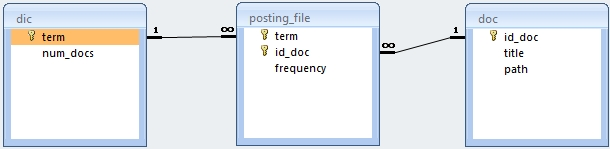
\includegraphics[keepaspectratio, scale=0.75]{./images/BD}
	\caption{Diagrama de la base de datos}
	\label{fig:BD}
\end{figure} 

Como sistema gestor de base de datos se ha optado por utilizar MySQL, ya que es ligero, libre, gratuito (ya que no se destina a fines comerciales) y compatible con otros sistemas, como Windows.

\subsection{Desarrollo del sistema}
Para terminar, en esta subsecci�n se comentan las diferentes decisiones de dise�o, as� como los problemas que han surgido a la hora de desarrollar el m�dulo de importaci�n e indexaci�n de documentos.

\subsubsection{Dise�o multicapa}
Este m�dulo se ha desarrollado siguiendo el enfoque multicapa, para desacoplar las operaciones del dominio de las operaciones de persistencia y presentaci�n, consiguiendo as� un sistema extensible y reutilizable.

Un ejemplo de la extensibilidad del sistema es que en la capa de presentaci�n se han implementado dos interfaces de usuario, una en modo gr�fico y otra por l�nea de comandos, tal y como se detallan en la secci�n \ref{manual}. 

En la capa de dominio, se almacenan las clases que implementan esta aplicaci�n, como son el analizador de los documentos y las clases auxiliares que utiliza, como las cach�s y un archivo de configuraci�n. Las clases de la capa de presentaci�n conocen a las clases de dominio (en concreto, al analizador), pero no al rev�s, por lo que podr�a cambiarse la interfaz de usuario sin tener que cambiar las clases de dominio.

Por otra parte, en la capa de persistencia se encuentran las clases que se encargan de almacenar la informaci�n en la base de datos. Dichas clases implementan un patr�n Agente Singleton y un patr�n fabricaci�n pura o DAO. El primer patr�n es el que se encarga de inicializar la conexi�n de la base de datos si no existe ya una instancia del agente, cerrar la conexi�n y ejecutar las sentencias sql que recibe del patr�n DAO. Dicho patr�n se ha utilizado para desacoplar el dominio de la persistencia, evitando as� que las propias clases del dominio creen las secuencias sql necesarias para gestionar la base de datos, pasando �sto a ser responsabilidad del patr�n DAO. Por tanto, si en alg�n momento se cambia el sistema gestor de base de datos, las clases de dominio no se ver�an afectadas, ya que s�lo habr�a que cambiar el agente y el DAO. 

\subsubsection{Analizador de documentos}

\paragraph{Conexi�n con la base de datos} En una primera iteraci�n del desarrollo de la aplicaci�n, la conexi�n con la base de datos se creaba cada vez que se quer�a acceder a ella, como, por ejemplo, al actualizar la frecuencia de un t�rmino en el \textit{posting$\_$file}, cerr�ndose al terminar el acceso. Esto consum�a mucho tiempo y el acceso a disco era muy elevado, por lo que se ha optado por inicializar la conexi�n con la base de datos al lanzar la apliaci�n, y cerrarla cuando la aplicaci�n finaliza.

\paragraph{Copia de documentos} Cuando se analiza un documento para realizar su indexaci�n, en un primer momento se copiaba el documento en la base de datos documental leyendo l�nea por l�nea. Este proceso era algo lento, por lo que finalmente se ha utilizado una llamada al sistema implementada en C, consiguiendo que la copia del documento completo sea instant�nea. 

\paragraph{Parser} Para realizar el tratamiento de los documentos y prepararlos para su indexaci�n, se ha implementado el m�todo \textit{parser}. Dicho m�dulo recibe una l�nea del documento a indexar y realiza la siguientes acciones: 
\begin{milista}
	\item En primer lugar, se escapan los caracteres ''$\backslash$'' y '' ' '' de las palabras que los contengan, ya que si se intenta insertar un t�rmino con esos caracteres, la sentencia sql no se forma de manera correcta y se provoca una excepci�n al ejecutar esa sentencia en la base de datos. 
	\item Se definen separadores de palabras, que son tanto los signos de puntuaci�n, como los espacios en blanco (incluyendo saltos de l�nea, tabuladores, etc). Se define tambi�n un patr�n para detectar direcciones IP.
	\item Se sustituyen las vocales acentuadas de las palabras por vocales sin acentuar.
	\item En cada una de las palabras de la l�nea, se sustituyen los separadores que pueda contener la palabra por un espacio en blanco, obteniendo as� una lista de palabras, que recibe el siguiente tratamiento:
	\begin{enumerate}
	\item Se eliminan los espacios en blanco.
	\item Si alguna palabra de la lista que se ha obtenido al dividir una palabra por separadores se encuentra en la stop$\_$list, dicha palabra no se divide, ya que quedar�an palabras sin sentido. Por ejemplo, si la palabra ''F-14'' se divide en ''[F,'' '',14]'', al encontrarse ''F'' en la stop$\_$list, se almacenar�a todo el t�rmino sin separarse.
	\item Si al dividir la palabra solo se obtiene una palabra de la stop$\_$list rodeada de espacios, dicha palabra se ignora. Por ejemplo, al separar la palabra ''$\backslash$t already?'', se obtendria la lista ['' '', '' '', already,'' ''], que solo contiene una palabra de la stop$\_$list rodeada de espacios, lo cual no tiene sentido. 
	\item En las direcciones web o de e-mail, el tratamiento es el mismo: se separa la palabra por seaparadores, obteniendo una lista y alamcenando las palabras por separado. Esto soluciona el siguiente problema: si el texto no tiene una escritura correcta y apareciese la palabra ''juanro.1987@gmail.com.Hola'', con este tratamiento se alamcenar�an las palabras ''juanro'', ''1987'', ''gmail'', ''com'' y ''hola''. Sin embargo, si tratasemos un e-mail como una palabra completa hasta que se encontrase un espacio, se almacenar�a como t�rmino ''juanro.1987@gmail.com.Hola'', que luego no se encontrar�a si alguien consulta por la direcci�n de e-mail ''juanro.1987@gmail.com''. En nuestro caso, como este mismo parser se va a aplicar a las consultas, la cadena anterior recibir�a el mismo tratamiento y podr�a recuperar los t�rminos que se hab�an almacenado por separado.
	\end{enumerate}
\end{milista}

\paragraph{Codificaci�n de documentos y de la base de datos} Tras realizar m�ltiples pruebas con diferentes documentos, se observaron fallos a la hora de recuperar y almacenar t�rminos en la base de datos. Estos fallos eran debidos a la codificaci�n de los documentos, que debe ser UTF-8 para el corrrecto funcionamiento en sistemas UNIX. Por tanto, todos los documentos de la colecci�n se han estandarizado a la codificaci�n UTF-8, al igual que las diferentes tablas de la base de datos.

\paragraph{Posting$\_$file} Se ha optado por almacenar el posting$\_$file de cada documento en memoria en forma de diccionario (tabla hash), para conseguir que los accesos sean m�s r�pidos. Se han realizado pruebas y para un documento de unas 25.000 l�neas, el tama�o del posting$\_$file no excede de los 13MB en memoria. Por tanto, esta opci�n es m�s eficiente en cuanto a tiempo que ir accediendo a la base de datos por cada uno de los t�rminos que se deben almacenar de cada uno de los documentos.


------------------
CACHE
PYSCO
HILOS EN GUI
FUTURAS MEJORAS
BIBLIOGRAFIA
------------------





\clearpage
\section{Manual de usuario} \label{manual}

\subsection{Instalaci�n}
La aplicaci�n se ha desarrollado en Python y su interfaz gr�fica de
usuario en GTK. Adem�s, �sta requiere de los servicios de un servidor
MySQL. Dicho esto, el sistema en el cual se ejecutar� la aplicaci�n
debe tener instalado el siguiente software:
\begin{milista}
\item Python v2.5 o superior (\cite{Python})
\item GTK (\cite{GTK})
\item Psyco (\cite{psyco})
\item PyGTK (\cite{PyGTK})
\item MySQL (\cite{MySQL})
\item MySQLdb module for Python (\cite{python-mysqldb})
\end{milista}

Inicialmente se debe crear la base de datos que utilizar� el sistema
documental. En la distribuci�n del software se ofrece un fichero
``install'' bajo el directorio ra�z, que contiene las
sentencias necesarias para crear la base de datos y sus tablas
mediante el int�rprete de MySQL. Para acceder al int�rprete de
su servidor MySQL escriba la siguiente sentencia en un terminal:

\begin{center} \texttt{mysql -u root -p} \end{center}

Introduzca la contrase�a que configur� al instalar el servidor de MySQL y cree las tablas con el fichero comentado anteriormente. Llegados a este punto, ya tiene su sistema listo para ser utilizado, pero antes es necesario destacar que �ste consiste en dos aplicaciones que pueden ser utilizadas de forma conjunta o por separado: un motor de indexaci�n y un motor de b�squeda. Cada motor posee su propia interfaz gr�fica de usuario independiente y, adicionalmente, el motor de indexaci�n posee una interfaz basada en l�nea de comandos.

\subsection{Motor de indexaci�n}
\subsubsection{Interfaz gr�fica de usuario}
Para ejecutar la interfaz gr�fica sit�ese en el directorio
''presentaci�n'' y ejecute la sentencia
\texttt{./indexEngineGUI.py}. A continuaci�n se mostrar� la ventana principal, tal
y como aparece en la Figura \ref{fig:index-engine-gui}. Las opciones de dicha
ventana son:
\begin{milista}
	\item \textbf{Choose a file}: esta opci�n sirve para indexar
          un �nico fichero. Al pulsar el bot�n, se abrir� un cuadro de
          di�logo que permitir� al usuario seleccionar el fichero deseado. 
	\item \textbf{Choose a directory}: esta opci�n sirve para
          indexar todos los ficheros contenidos en el directorio
          dado. Al pulsar el bot�n correspondiente, se abrir� un nuevo
          di�logo que permitir� al usuario elegir un directorio. 
\end{milista}

\begin{figure}[h]
	\centering
		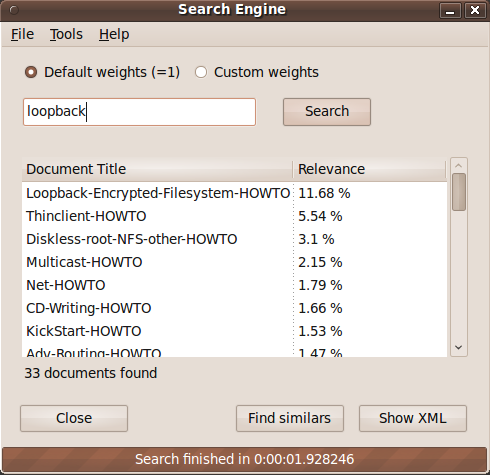
\includegraphics[keepaspectratio, scale=0.75]{./images/index-engine-gui}
	\caption{Interfaz gr�fica de usuario del motor de indexaci�n}
	\label{fig:index-engine-gui}
\end{figure} 

Una vez elegido un fichero o un directorio, basta con hacer clic en el
bot�n ''Start'' para que comienze la indexaci�n, mostrando una
barra de progreso para informar al usuario del avance de la indexaci�n de los
ficheros. 

\subsubsection{Interfaz de usuario por l�nea de comandos}
El m�dulo de indexaci�n adem�s cuenta con una interfaz basada en texto que puede
invocarse desde un terminal. Una vez m�s, esta interfaz est� contenida
en la capa de presentaci�n del sistema, por lo que hay que introducir la sentencia (\texttt{./indexEngineCMD.py}), siendo necesario
proporcionarle dos par�metros, en funci�n de la operaci�n que queramos
realizar.
\begin{milista}
\item \texttt{[-f | --file] <ruta$\_$a$\_$un$\_$fichero>}. Para indexar un �nico fichero.
\item \texttt{[-d | --directory] <ruta$\_$a$\_$un$\_$directorio>}. Para indexar todos
  los ficheros alojados en un directorio
\end{milista}
Si es necesario, se puede consultar la ayuda con el par�metro ``-h'' o
``--help'' (ver Figura \ref{fig:menu-ayuda})

\begin{figure}[h]
	\centering
		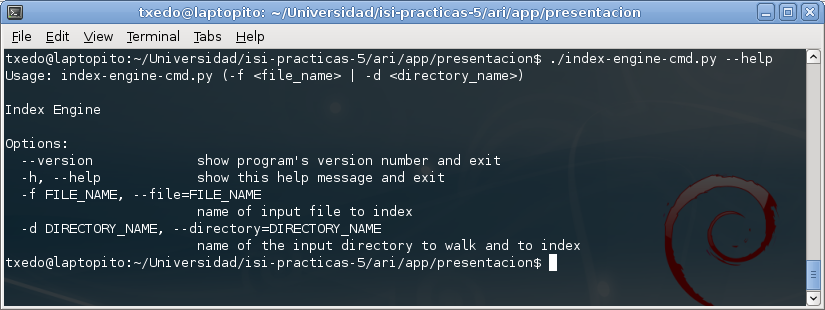
\includegraphics[keepaspectratio, scale=0.55]{./images/menu-ayuda}
	\caption{Ayuda para el motor de indexaci�n usando l�nea de comandos}
	\label{fig:menu-ayuda}
\end{figure}

\subsection{Motor de b�squeda}
Debido a las funcionalidades que debe cubrir esta aplicaci�n, se proporciona una interfaz gr�fica de usuario (ver Figura \ref{fig:search-engine-gui}). Para ejecutarla, escriba en su terminal la sentencia \texttt{./searchEngineGUI.py} una vez que se haya situado en el directorio ``presentacion'' de la aplicaci�n.

\begin{figure}[h]
	\centering
		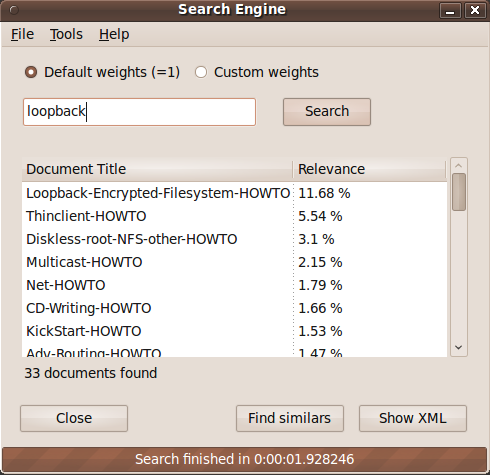
\includegraphics[keepaspectratio, scale=0.55]{./images/search-engine-gui}
	\caption{Interfaz gr�fica de usuario del motor de b�squeda}
	\label{fig:search-engine-gui}
\end{figure}

En cuanto a las caracter�sticas de esta aplicaci�n cabe destacar las siguientes caracter�sticas:
\begin{milista}
\item Se puede invocar el motor de b�squeda a partir del men� ''Tools''.
\item En el men� ''Tools'' se pueden consultar los documentos indexados en el sistema (ver Figura \ref{fig:indexedDocuments}) y ver su contenido, haciendo doble clic en uno de ellos, o pulsando ENTER al seleccionarlo.
\begin{figure}[h]
	\centering
		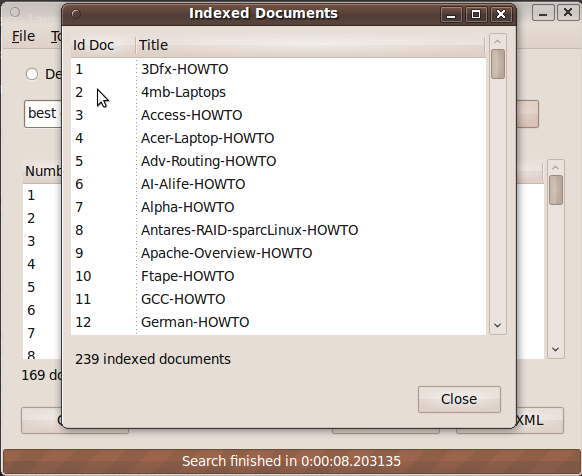
\includegraphics[keepaspectratio, scale=0.55]{./images/indexedDocuments}
	\caption{Di�logo que muestra los documentos indexados en el sistema}
	\label{fig:indexedDocuments}
\end{figure}
\item A la hora de realizar una b�squeda podemos configurar los pesos que deseamos dar a cada t�rmino. Por defecto, cada t�rmino tendr� peso 1, que es el m�ximo que puede tener, de modo que si queremos quitarle importancia a un t�rmino debemos indicarle un peso entre 0 y 1 mediante su barra deslizante correspondiente. Otra caracter�stica importante del sistema es que nos permitir� configurar los pesos sobre los t�rmios que realmente formar�n parte de la pregunta, ignorando \textit{stopwords} y parseando el texto (ver Figura \ref{fig:custom-weights}).
\begin{figure}[h]
	\centering
		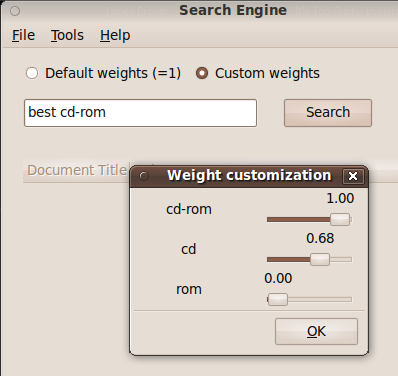
\includegraphics[keepaspectratio, scale=0.55]{./images/custom-weights}
	\caption{Configurando los pesos a los t�rminos parseados de una pregunta e ignorando stopwords}
	\label{fig:custom-weights}
\end{figure}
\item Una vez que hemos realizado una b�squeda, se muestran los documentos encontrados ordenados de mayor a mener relevancia con respecto a la pregunta introducida. Adem�s, si hacemos doble clic sobre un documento o lo seleccionamos y presionamos la tecla ENTER, emerger� una ventana mostr�ndonos su contenido (ver Figura \ref{fig:dialogoTexto}).
\begin{figure}[h]
	\centering
		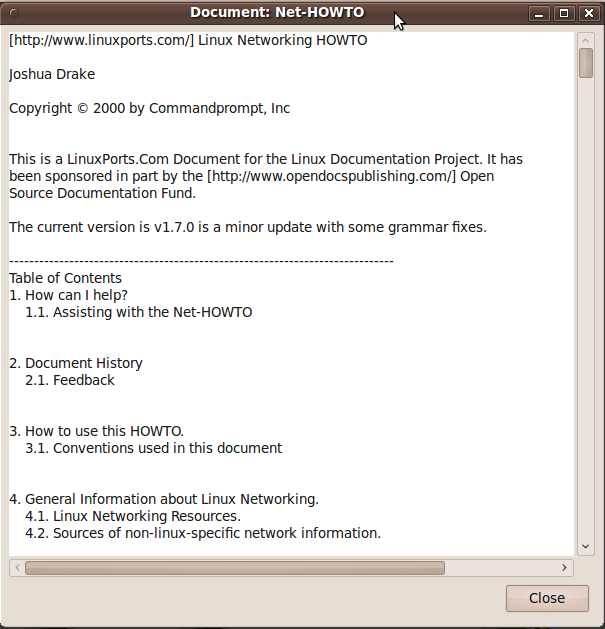
\includegraphics[keepaspectratio, scale=0.55]{./images/dialogoTexto}
	\caption{Di�logo que muestra el texto del documento seleccionado}
	\label{fig:dialogoTexto}
\end{figure}
\item Tambi�n podemos buscar documentos similares al documento que tengamos seleccionado. Para ello haremos uso del bot�n ''Find similars''.
\item Por �ltimo, los resultados tambien pueden ser visualizados en el navegador configurado por defecto en el sistema (ver Figura \ref{fig:firefox}). Para ello haremos uso del boton ''Show XML''.
\begin{figure}[h]
	\centering
		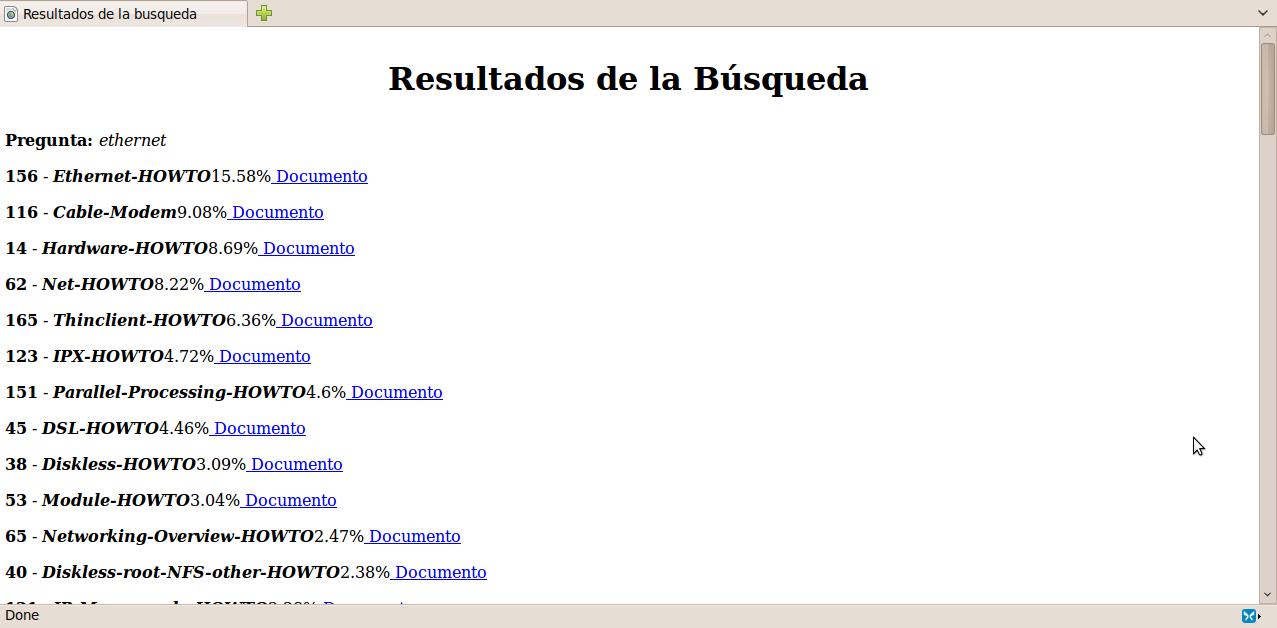
\includegraphics[keepaspectratio, scale=0.35]{./images/firefox}
	\caption{Resultado de la b�squeda mostrado en el navegador Web}
	\label{fig:firefox}
\end{figure}

\end{milista}

\clearpage
\section{Estad�sticas de funcionamiento} \label{estadisticas}

Las pruebas se han realizado en un sistema Debian GNU/Linux 4.0
Etch sobre un ordenador Centrino@2.0GHz FSB800MHz 2.0GB RAM
DRR2@800MHz.

El conjunto de ficheros de muestra se compone de un total de 239.

Ya sea utilizando una memoria cach� de tama�o 1 (caso base, comportamiento
similar al de un sistema sin cach�) como de tama�o 1000, el tiempo
que se ha obtenido en la indexaci�n es similar: entorno a los 27
minutos. La diferencia radica en que en el primer caso el acceso a
disco y el uso del procesador se mantiene constante, mientras que en
el segundo caso ambos usos de recursos vienen dados por intevalos,
coincidiendo �stos con la sincronizaci�n de la cach� con la base de
datos.

No obstante, estos resultados nos hacen meditar en que el uso de la
memoria cach� no ha mejorado la eficiencia del sistema tanto como se
esperaba, por lo que en pr�ximas versiones se har�n las revisiones
pertinentes.

\clearpage

\end{document}
